\documentclass[12pt, a4paper]{article}

% ── Packages ──────────────────────────────────────────────────────────────────
\usepackage[margin=2.5cm, top=3cm, bottom=3cm]{geometry}
\usepackage[table]{xcolor}
\usepackage{amsmath}
\usepackage{booktabs}
\usepackage{array}
\usepackage{tabularx}
\usepackage{graphicx}
\usepackage{hyperref}
\usepackage{fancyhdr}
\usepackage{titlesec}
\usepackage{parskip}
\usepackage{enumitem}
\usepackage[letterspace=150]{microtype}
\usepackage{mdframed}
\usepackage{lmodern}
\usepackage{fontenc}
\usepackage{inputenc}
\usepackage{caption}
\usepackage{subcaption}
\usepackage{float}
\usepackage{multirow}
\usepackage{longtable}
\usepackage{tcolorbox}
\tcbuselibrary{skins, breakable}

% ── Colours ───────────────────────────────────────────────────────────────────
\definecolor{ehaBlue}{RGB}{0, 84, 142}
\definecolor{ehaLightBlue}{RGB}{224, 237, 248}
\definecolor{ehaGrey}{RGB}{245, 245, 245}
\definecolor{ehaAccent}{RGB}{0, 153, 118}
\definecolor{ehaRed}{RGB}{192, 57, 43}
\definecolor{ehaAmber}{RGB}{230, 126, 34}
\definecolor{tableHead}{RGB}{0, 84, 142}
\definecolor{tableAlt}{RGB}{240, 248, 255}

% ── Hyperlinks ─────────────────────────────────────────────────────────────────
\hypersetup{
  colorlinks=true, linkcolor=ehaBlue, urlcolor=ehaBlue,
  pdftitle={EDA Report: EHA Clinics Procurement Data},
  pdfauthor={Supply Chain Analytics},
}

% ── Header / Footer ───────────────────────────────────────────────────────────
\pagestyle{fancy}
\fancyhf{}
\fancyhead[L]{\small\textcolor{ehaBlue}{\textbf{EHA Clinics} $\mid$ Procurement EDA Report}}
\fancyhead[R]{\small\textcolor{gray}{April 2026}}
\fancyfoot[C]{\small\textcolor{gray}{\thepage}}
\renewcommand{\headrulewidth}{0.4pt}
\renewcommand{\headrule}{\hbox to\headwidth{\color{ehaBlue}\leaders\hrule height\headrulewidth\hfill}}
\setlength{\headheight}{24pt}

% ── Section styling ───────────────────────────────────────────────────────────
\titleformat{\section}{\large\bfseries\color{ehaBlue}}{\thesection.}{0.6em}{}[\titlerule]
\titleformat{\subsection}{\normalsize\bfseries\color{ehaBlue!80!black}}{\thesubsection}{0.6em}{}
\titlespacing*{\section}{0pt}{1.6em}{0.7em}
\titlespacing*{\subsection}{0pt}{1.1em}{0.4em}

% ── Callout boxes ─────────────────────────────────────────────────────────────
\mdfdefinestyle{keybox}{
  backgroundcolor=ehaLightBlue, linecolor=ehaBlue, linewidth=1pt,
  innerleftmargin=12pt, innerrightmargin=12pt,
  innertopmargin=10pt, innerbottommargin=10pt, roundcorner=4pt,
}
\mdfdefinestyle{warnbox}{
  backgroundcolor=ehaAmber!12, linecolor=ehaAmber, linewidth=1.5pt,
  topline=false, rightline=false, bottomline=false,
  innerleftmargin=12pt, innerrightmargin=12pt,
  innertopmargin=8pt, innerbottommargin=8pt,
}
\mdfdefinestyle{alertbox}{
  backgroundcolor=ehaRed!8, linecolor=ehaRed, linewidth=1.5pt,
  topline=false, rightline=false, bottomline=false,
  innerleftmargin=12pt, innerrightmargin=12pt,
  innertopmargin=8pt, innerbottommargin=8pt,
}
\mdfdefinestyle{greenbox}{
  backgroundcolor=ehaAccent!10, linecolor=ehaAccent, linewidth=1.5pt,
  topline=false, rightline=false, bottomline=false,
  innerleftmargin=12pt, innerrightmargin=12pt,
  innertopmargin=8pt, innerbottommargin=8pt,
}

% ── Table helpers ─────────────────────────────────────────────────────────────
\newcolumntype{L}[1]{>{\raggedright\arraybackslash}p{#1}}
\newcolumntype{C}[1]{>{\centering\arraybackslash}p{#1}}
\newcolumntype{R}[1]{>{\raggedleft\arraybackslash}p{#1}}

% ── Figure caption style ──────────────────────────────────────────────────────
\captionsetup{font=small, labelfont={bf,color=ehaBlue}, labelsep=period,
              skip=6pt, width=0.95\textwidth}

% ── Finding counter ───────────────────────────────────────────────────────────
\newcounter{finding}
\newcommand{\finding}[1]{%
  \stepcounter{finding}%
  \begin{mdframed}[style=greenbox]
  \textbf{Finding \thefinding:} #1
  \end{mdframed}%
}

\begin{document}

% ════════════════════════════════════════════════════════════════════════════════
%  TITLE PAGE
% ════════════════════════════════════════════════════════════════════════════════
\begin{titlepage}
  \pagecolor{ehaBlue}\color{white}
  \vspace*{1.8cm}

  {\fontsize{10}{12}\selectfont\MakeUppercase{\textls[100]{Analytical Report}}}\\[0.5em]
  {\fontsize{26}{32}\selectfont\bfseries Exploratory Data Analysis\\[0.3em]
   of Procurement Records}\\[1.2em]
  \textcolor{ehaAccent}{\rule{6cm}{2pt}}\\[1.2em]

  {\large Procurement Demand Forecasting Initiative}\\[0.4em]
  {\normalsize EHA Clinics $\cdot$ Supply Chain Analytics}\\[2.5cm]

  \begin{tabular}{@{}ll}
    \textbf{Document Version} & 1.0 \\[0.4em]
    \textbf{Date}             & April 30, 2026 \\[0.4em]
    \textbf{Data source}      & Odoo ERP (exported CSV) \\[0.4em]
    \textbf{Analysis window}  & 2018 -- 2024 (training: 2021--2023) \\[0.4em]
    \textbf{Status}           & Final \\
  \end{tabular}

  \vfill
  {\small\textcolor{white!70!ehaBlue}
    {This report presents the results of an exploratory analysis of EHA Clinics'
     historical procurement data, establishing the factual evidence base for
     the demand forecasting model and identifying data quality issues,
     demand patterns, seasonality, and series forecastability before modelling begins.}}
\end{titlepage}
\pagecolor{white}\color{black}

% ════════════════════════════════════════════════════════════════════════════════
%  EXECUTIVE SUMMARY
% ════════════════════════════════════════════════════════════════════════════════
\newpage

\begin{mdframed}[style=keybox]
\textbf{\large Executive Summary}\\[0.6em]
This exploratory analysis examined \textbf{43,799 procurement records} from
EHA Clinics' Odoo ERP system spanning 2018 to 2024, covering 16 branch
locations across Abuja, Kano, and Lagos. After filtering to confirmed
(\texttt{done}) orders for in-scope health commodity categories at the six
designated pilot facilities, the working analytical dataset comprises
\textbf{8,965 records}.\\[0.5em]

Five key findings emerge:
\begin{enumerate}[leftmargin=1.5em, itemsep=3pt]
  \item \textbf{Data is largely usable but has meaningful quality gaps:}
        12.4\% of records have no branch assignment; 2.1\% have zero quantity.
        These are well-understood limitations that are addressable through
        the filtering strategy defined in the Scope Note.
  \item \textbf{A single bulk stock-load event dominates the 2021 data:}
        The Kano -- Independence Road facility recorded 258,470 units in
        September 2021 alone, representing a one-time distribution stock-loading
        event, not clinical demand. This facility requires special treatment.
  \item \textbf{Forecast readiness varies considerably across pairs:}
        Prescription Medications and OTC Drugs at Asba and Kano Lamido are
        data-rich ($\geq$30 non-zero months); Dental Consumables and NPI
        Vaccines are severely sparse across most facilities.
  \item \textbf{Seasonality is present but varies by category:}
        OTC Drugs and Injections show Q4 demand peaks consistent with
        Nigeria's dry-season respiratory illness burden; Vaccines are
        more evenly distributed with slight Q2 elevations.
  \item \textbf{Laboratory Consumables carry the highest unit cost:}
        Despite ranking fifth by volume, this category accounts for the
        highest total spend (NGN 83M), pointing to significant financial
        risk from forecast errors in this category.
\end{enumerate}
\end{mdframed}

\newpage
\tableofcontents
\newpage

% ════════════════════════════════════════════════════════════════════════════════
%  1. INTRODUCTION
% ════════════════════════════════════════════════════════════════════════════════
\section{Introduction}

Exploratory Data Analysis (EDA) is the necessary first step before any
forecasting model is built. Its purpose is threefold: to characterise the
data as it actually exists (not as assumed), to surface quality issues that
must be resolved before training, and to generate evidence-based expectations
about what modelling approaches are likely to work --- and where.

This report covers the full analytical pipeline from raw data ingestion
through to a quantified forecast-readiness assessment per
category-facility pair. The findings directly inform the modelling strategy
described in the Forecasting Scope and Modelling Approach concept note.

\subsection{Dataset Description}

The source dataset is a flat export from EHA Clinics' Odoo ERP system,
containing one row per purchase order line item. Each record captures the
ordering facility (\texttt{branch\_name}), product and category
(\texttt{product\_name}, \texttt{category\_name}), quantity and value
(\texttt{product\_qty}, \texttt{price\_subtotal}), and timing
(\texttt{date\_order}, \texttt{month}, \texttt{quarter}, \texttt{year}).

\vspace{0.6em}
\noindent
\begin{tabularx}{\textwidth}{@{} L{4cm} X @{}}
  \toprule
  \rowcolor{tableHead}
  \textcolor{white}{\textbf{Field}} & \textcolor{white}{\textbf{Description}} \\
  \midrule
  \texttt{order\_id}          & Unique purchase order identifier \\
  \rowcolor{tableAlt}
  \texttt{branch\_name}       & Facility that raised the order \\
  \texttt{product\_name}      & Full product description \\
  \rowcolor{tableAlt}
  \texttt{category\_name}     & Procurement category \\
  \texttt{product\_qty}       & Quantity ordered \\
  \rowcolor{tableAlt}
  \texttt{price\_subtotal}    & Total line value (NGN) \\
  \texttt{state}              & Order status (\texttt{done} / \texttt{purchase}) \\
  \rowcolor{tableAlt}
  \texttt{month}              & Month of order (truncated to first of month) \\
  \bottomrule
\end{tabularx}

% ════════════════════════════════════════════════════════════════════════════════
%  2. DATA QUALITY ASSESSMENT
% ════════════════════════════════════════════════════════════════════════════════
\section{Data Quality Assessment}

\subsection{Overview of Issues}

Figure~\ref{fig:quality} presents the data quality issues identified across
all 43,799 records. The most significant issue is \textbf{missing branch
names} (5,427 records, 12.4\%), which renders those rows unusable for
facility-level demand forecasting. Investigation reveals that these correspond
predominantly to early records (2018--2019) and a small number of
centrally-raised orders that were not assigned to a specific branch in Odoo.

\begin{figure}[H]
  \centering
  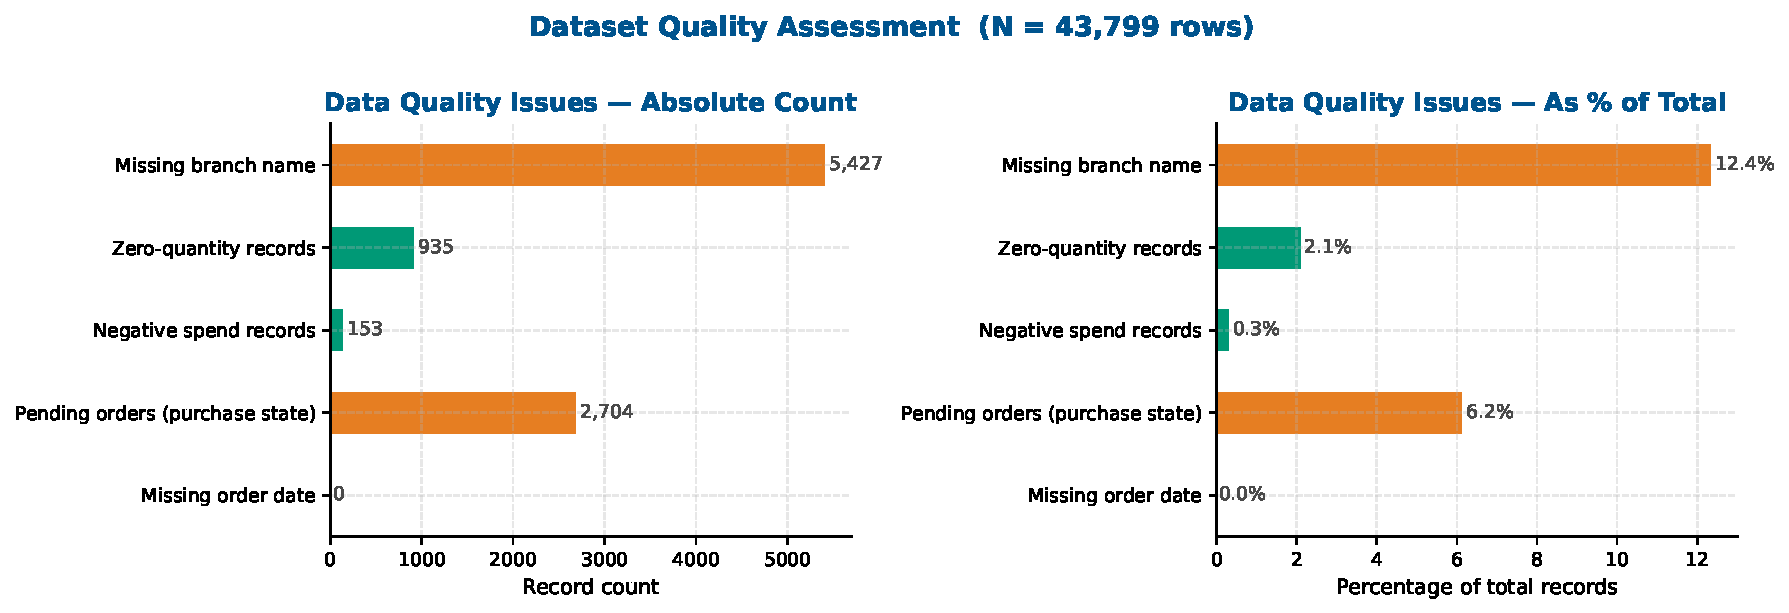
\includegraphics[width=0.95\textwidth]{figures/fig1_data_quality.pdf}
  \caption{Data quality issues across all 43,799 procurement records.
           Amber bars indicate counts exceeding 1,000 records (material
           impact); green bars indicate minor issues.}
  \label{fig:quality}
\end{figure}

\vspace{0.4em}
\noindent
\begin{tabularx}{\textwidth}{@{} L{4.8cm} R{1.8cm} R{1.8cm} X @{}}
  \toprule
  \rowcolor{tableHead}
  \textcolor{white}{\textbf{Issue}} &
  \textcolor{white}{\textbf{Count}} &
  \textcolor{white}{\textbf{\% of Total}} &
  \textcolor{white}{\textbf{Resolution}} \\
  \midrule
  Missing branch name     & 5,427 & 12.4\% & Excluded from facility models \\
  \rowcolor{tableAlt}
  Pending state (\texttt{purchase}) & 2,704 & 6.2\% & Excluded (use \texttt{done} only) \\
  Zero-quantity records   & 935   & 2.1\% & Treated as non-events; excluded from training \\
  \rowcolor{tableAlt}
  Negative spend records  & 153   & 0.3\% & Credit notes / discounts; excluded \\
  Missing order date      & $<$5  & $<$0.1\% & Negligible; excluded \\
  \bottomrule
\end{tabularx}

\vspace{0.8em}

\finding{Data quality issues are significant in absolute count but well-understood
in origin. After applying the defined filters (\texttt{state = done},
non-zero quantity, branch assigned, in-scope category, pilot facility),
the working analytical dataset retains \textbf{8,965 records} --- sufficient
for category-level modelling but requiring careful handling at the
category-facility pair level.}

\subsection{Implications for Modelling}

Zero-quantity records (935 rows) are particularly relevant to forecasting.
They arise from two distinct causes: \textbf{(a)} confirmed orders that were
later cancelled at the line level within Odoo, and \textbf{(b)} orders placed
against a product that was ultimately substituted with a different SKU.
Both cases represent true ``no-procurement'' events but are not necessarily
zero-demand events. The forecasting model must therefore be trained on
\textit{observed procurement quantities} while acknowledging that zeros in
the series may understate true clinical demand.

% ════════════════════════════════════════════════════════════════════════════════
%  3. TEMPORAL COVERAGE
% ════════════════════════════════════════════════════════════════════════════════
\section{Temporal Coverage and the 2021 Anomaly}

\subsection{Annual Procurement Trend}

Figure~\ref{fig:annual} shows annual procurement volume and spend for the
in-scope categories at pilot facilities from 2020 to 2024. The 2021 bar
is dramatically elevated --- 453,837 units, compared to 32,000--61,000 in
all other years. This is not a genuine demand surge.

\begin{figure}[H]
  \centering
  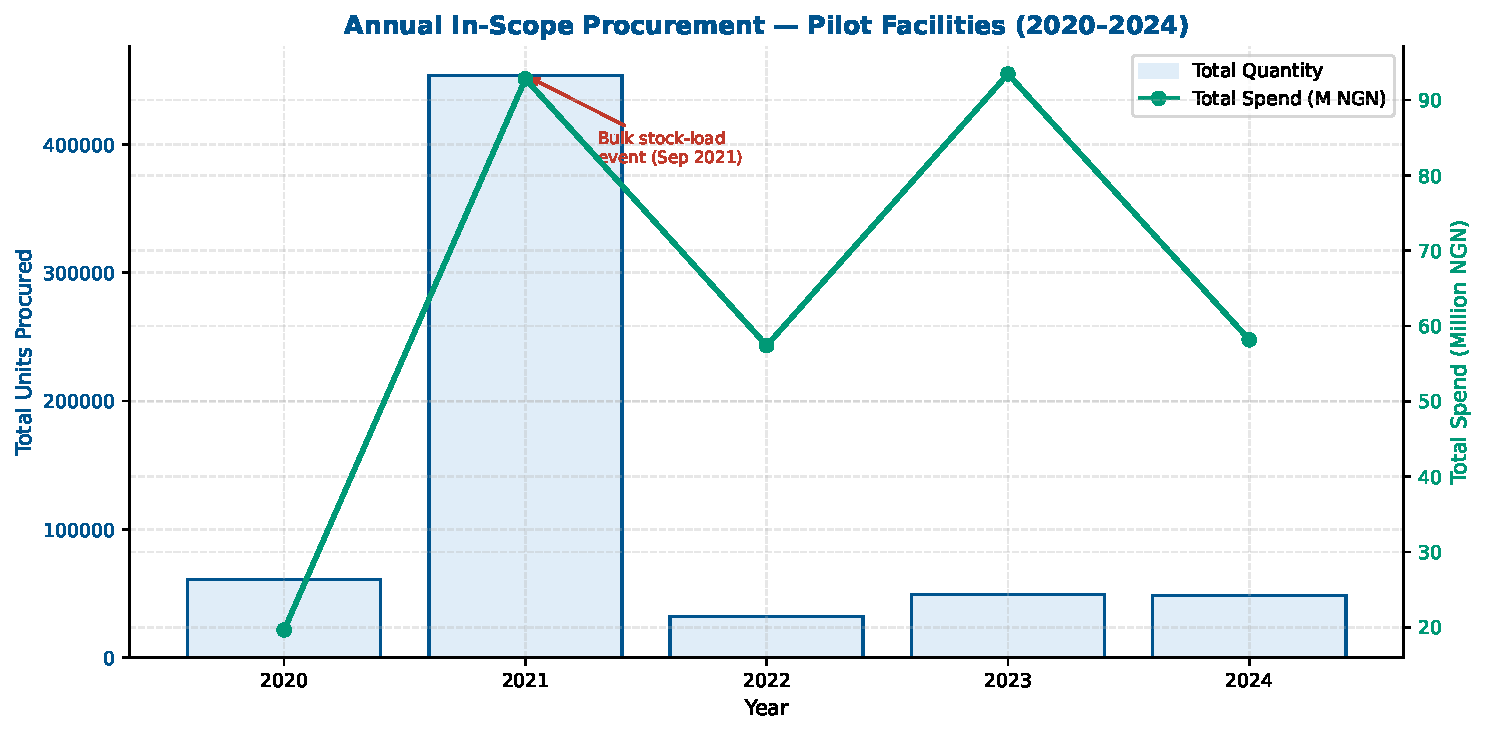
\includegraphics[width=0.92\textwidth]{figures/fig2_annual_trend.pdf}
  \caption{Annual in-scope procurement volume (bars) and total spend (line)
           at pilot facilities, 2020--2024. The 2021 spike is driven by a
           single bulk stock-load event at Kano -- Independence Road in
           September 2021.}
  \label{fig:annual}
\end{figure}

\subsection{The Kano Independence Road Bulk Event}

Figure~\ref{fig:kano} drills into the Kano -- Independence Road monthly
series and its September 2021 product breakdown.

\begin{figure}[H]
  \centering
  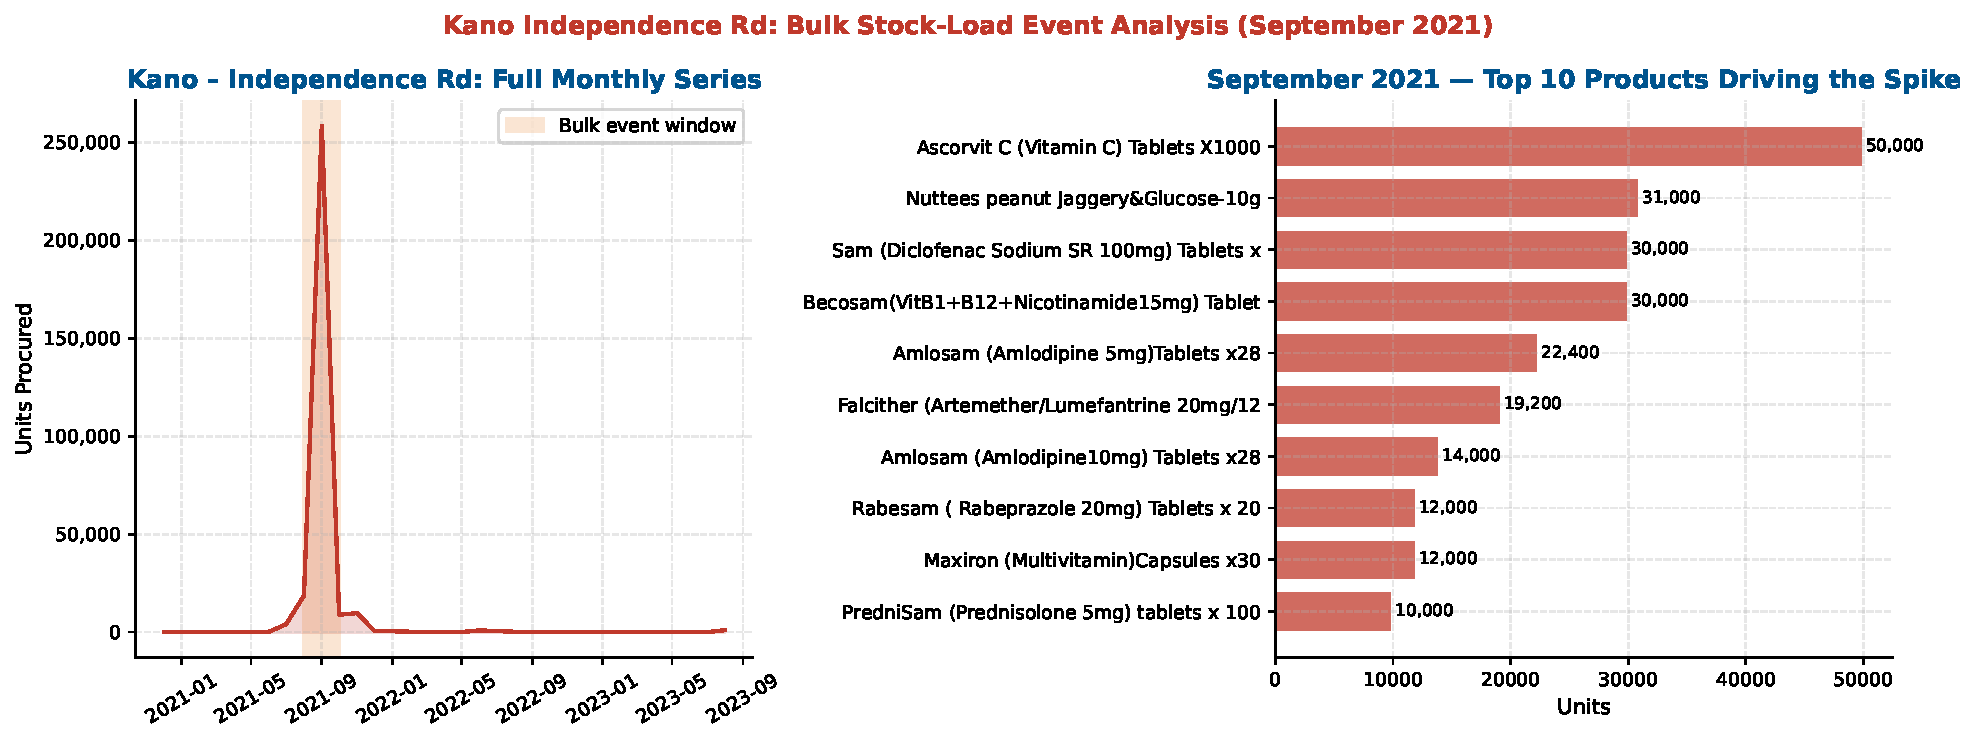
\includegraphics[width=0.95\textwidth]{figures/fig10_kano_anomaly.pdf}
  \caption{Left: Full monthly procurement series for Kano -- Independence Rd,
           showing the September 2021 spike of 258,470 units against a
           normal monthly baseline of 700--20,000 units. Right: The top 10
           products driving the spike, all of which are bulk OTC and
           prescription medications consistent with a distribution
           stock-loading exercise.}
  \label{fig:kano}
\end{figure}

The September 2021 event was driven by 10 products accounting for
$>$250,000 units in a single month (Table~\ref{tab:spike}). All are
high-volume, low-cost commodities consistent with a central stock-loading
exercise for EHA Pharma's distribution operations --- not routine
clinic-level clinical demand.

\vspace{0.5em}
\noindent
\begin{tabularx}{\textwidth}{@{} L{7cm} R{2.5cm} L{3.5cm} @{}}
  \toprule
  \rowcolor{tableHead}
  \textcolor{white}{\textbf{Product}} &
  \textcolor{white}{\textbf{Units (Sep 2021)}} &
  \textcolor{white}{\textbf{Category}} \\
  \midrule
  Ascorvit C (Vitamin C) Tabs x1000   & 50,000 & OTC Drugs \\
  \rowcolor{tableAlt}
  Nuttees Peanut Jaggery \& Glucose   & 31,000 & OTC Drugs \\
  Sam (Diclofenac SR 100mg) x100      & 30,000 & OTC Drugs \\
  \rowcolor{tableAlt}
  Becosam (B-Vitamins) x1000          & 30,000 & Prescription Meds \\
  Amlosam (Amlodipine 5mg) x28        & 24,640 & Prescription Meds \\
  \rowcolor{tableAlt}
  Falcither (ACT 20/120mg) x24        & 24,000 & Prescription Meds \\
  Amlosam (Amlodipine 10mg) x28       & 14,280 & Prescription Meds \\
  \rowcolor{tableAlt}
  Maxiron (Multivitamin) x30          & 13,500 & OTC Drugs \\
  Rabesam (Rabeprazole 20mg) x20      & 12,000 & OTC Drugs \\
  \rowcolor{tableAlt}
  PredniSam (Prednisolone 5mg) x100   & 10,000 & Prescription Meds \\
  \midrule
  \textbf{Total}                      & \textbf{239,420} & \\
  \bottomrule
\end{tabularx}
\vspace{0.3em}
\captionof{table}{Top 10 products driving the Kano -- Independence Rd
September 2021 bulk procurement event.}
\label{tab:spike}

\vspace{0.8em}

\begin{mdframed}[style=alertbox]
\textbf{Modelling implication:} The Kano -- Independence Road 2021 data
must be excluded from the training window, or treated as a structural
break requiring explicit modelling. Leaving it in the training data would
severely overestimate normal demand at this facility and distort seasonal
pattern extraction across any model applied to this series.
\end{mdframed}

\finding{Kano -- Independence Road functioned as a distribution staging
point in 2021, not solely as a clinical demand site. Its 2021 records
are excluded from all model training. Post-2021 data for this facility
shows a normal per-clinic demand pattern (700--9,000 units/month) and
remains in scope.}

% ════════════════════════════════════════════════════════════════════════════════
%  4. FACILITY PROFILES
% ════════════════════════════════════════════════════════════════════════════════
\section{Facility Profiles}

Figure~\ref{fig:facility} compares the six pilot facilities across spend,
volume, and procurement activity, with the Kano Independence Road 2021
bulk event excluded.

\begin{figure}[H]
  \centering
  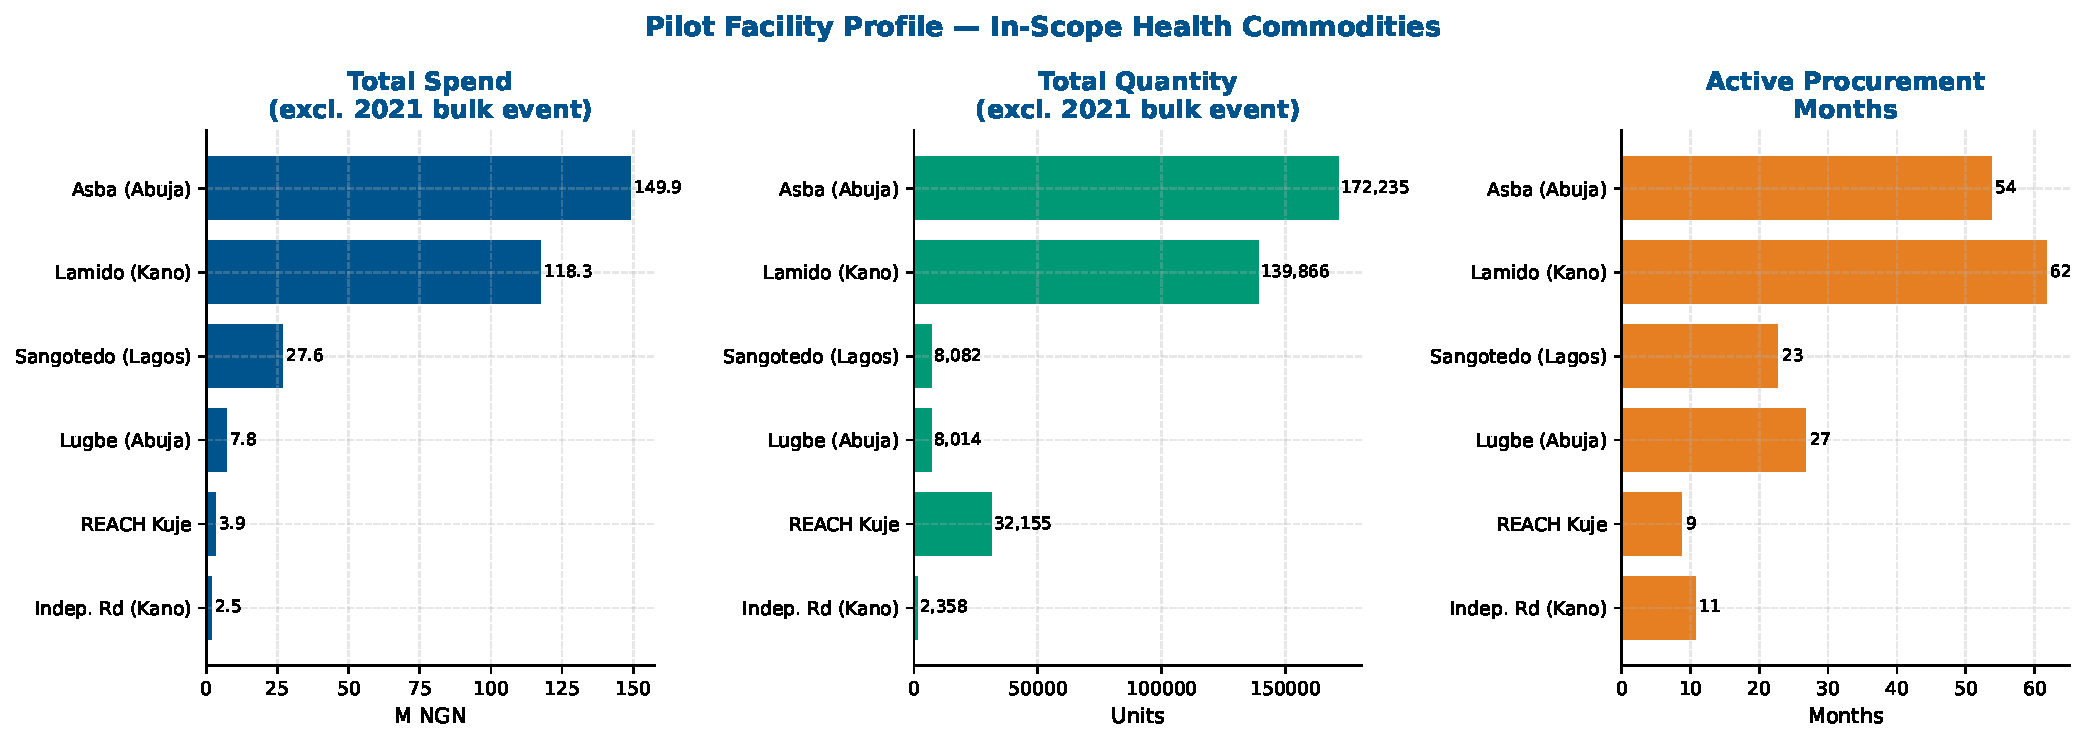
\includegraphics[width=\textwidth]{figures/fig3_facility_profile.pdf}
  \caption{Pilot facility comparison: total spend (left), total units
           procured (centre), and number of active procurement months
           (right). Kano Independence Rd 2021 bulk event excluded.}
  \label{fig:facility}
\end{figure}

\subsection{Key Observations}

\paragraph{Asba (Abuja) is the anchor facility.}
Abuja -- Asba and Dantata accounts for NGN~149.9M in in-scope spend ---
more than all other pilot facilities combined. It also has the longest
procurement history (53+ active months) and is the primary data source
for all category-facility pairs. Forecasts for this facility will have
the highest statistical confidence.

\paragraph{Kano -- Lamido Crescent is the second anchor.}
Lamido Crescent contributes NGN~118.3M in spend with 53 active months,
and is the highest-volume Kano facility after the Independence Road
bulk event is removed. Its demand profile likely reflects both urban
and referral clinic characteristics.

\paragraph{REACH Kuje and Lugbe are structurally different.}
REACH Kuje and Abuja -- Lugbe together account for less than 8\% of
total in-scope spend. These are community-facing facilities with
different commodity mixes and lower transaction frequencies. They will
require lower-complexity models (Seasonal Na\"{i}ve or ETS) rather than
SARIMA, which needs longer series.

\paragraph{Lagos -- Sangotedo Ajah is geographically isolated.}
Lagos is the only facility outside the Abuja-Kano corridor. It has
a moderate spend profile (NGN~27.6M) but fewer active procurement months
than the Kano and Abuja sites, reflecting the later establishment of this
facility. Its demand patterns may differ due to a different disease burden
and patient demography.

\vspace{0.5em}
\noindent
\begin{tabularx}{\textwidth}{@{} L{4.5cm} R{2.3cm} R{2.3cm} C{2.3cm} @{}}
  \toprule
  \rowcolor{tableHead}
  \textcolor{white}{\textbf{Facility}} &
  \textcolor{white}{\textbf{Spend (M NGN)}} &
  \textcolor{white}{\textbf{Volume (units)}} &
  \textcolor{white}{\textbf{Active months}} \\
  \midrule
  Asba and Dantata        & 149.9 & 56,792 & 53 \\
  \rowcolor{tableAlt}
  Kano -- Lamido Crescent & 118.3 & 53,406 & 53 \\
  Lagos -- Sangotedo Ajah & 27.6  & 8,082  & 31 \\
  \rowcolor{tableAlt}
  Kano -- Independence Rd & 23.6  & 19,684 & 14 \\
  Abuja -- Lugbe          & 7.8   & 8,014  & 28 \\
  \rowcolor{tableAlt}
  REACH Abuja -- Kuje     & 3.9   & 32,155 & 19 \\
  \bottomrule
\end{tabularx}
\vspace{0.3em}
\captionof{table}{Pilot facility profiles, in-scope health commodities
(2020--2024, Kano Indep. Rd 2021 bulk event excluded).}

% ════════════════════════════════════════════════════════════════════════════════
%  5. CATEGORY PROFILES
% ════════════════════════════════════════════════════════════════════════════════
\section{Category Profiles}

\subsection{Spend and Volume Distribution}

Figure~\ref{fig:category} presents the in-scope categories ranked by spend
and volume separately. The divergence between the two rankings reveals
important commodity economics.

\begin{figure}[H]
  \centering
  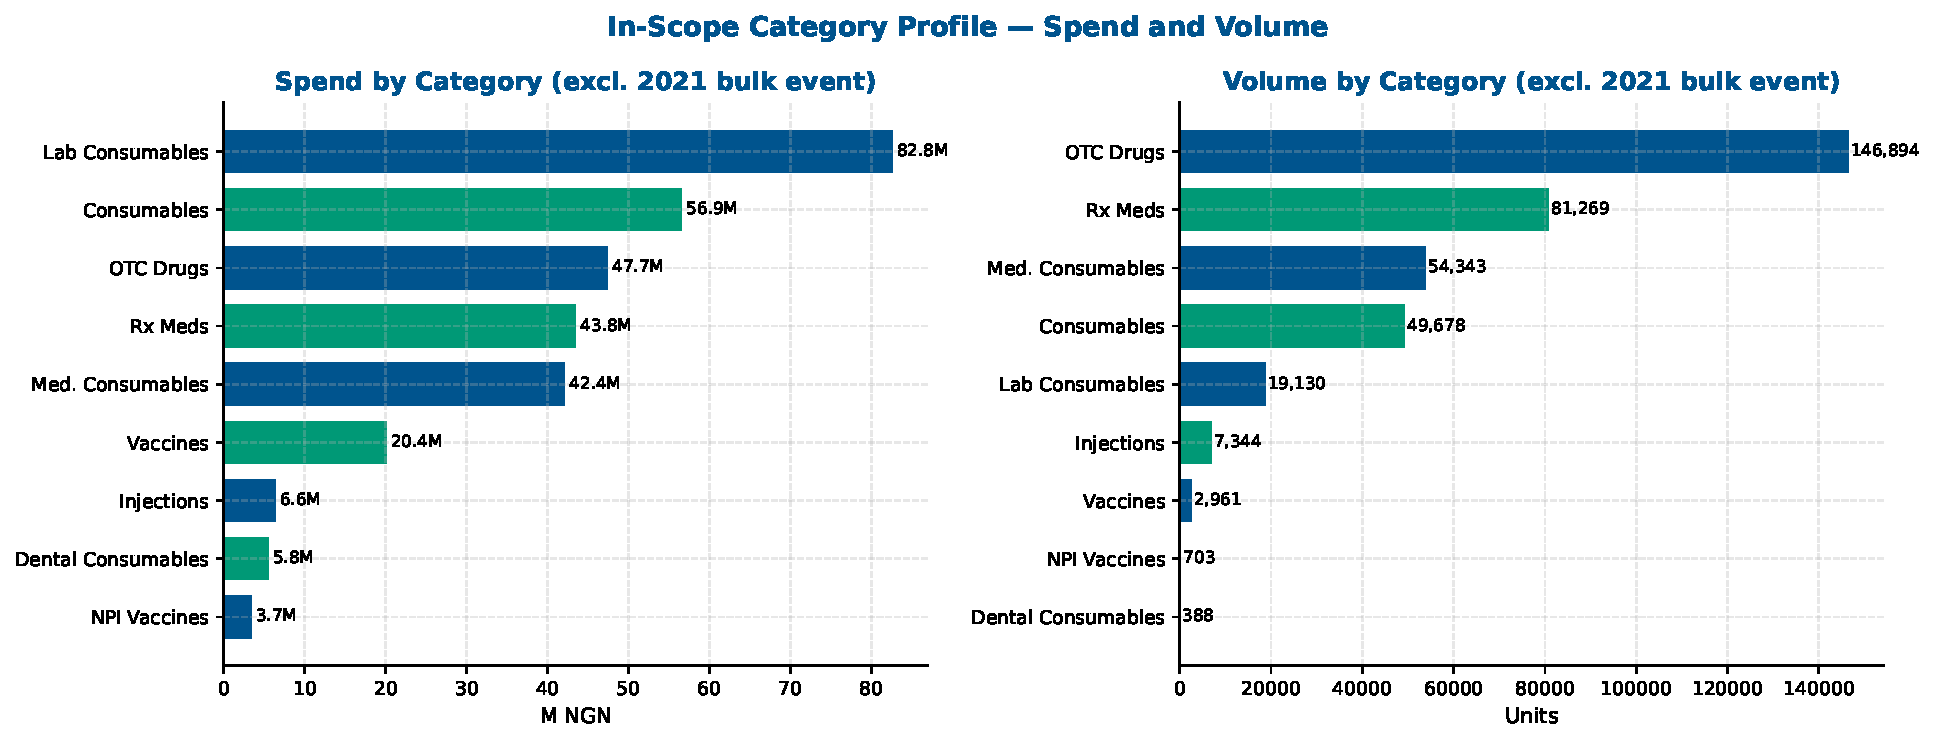
\includegraphics[width=\textwidth]{figures/fig4_category_profile.pdf}
  \caption{In-scope category comparison: total spend in M NGN (left) and
           total units procured (right), pilot facilities 2020--2024
           with the 2021 bulk event excluded.}
  \label{fig:category}
\end{figure}

\subsection{Category Economics}

\paragraph{Over The Counter Drugs and Consumables dominate by spend.}
Both categories carry approximately NGN~57M in spend, but for very
different reasons. OTC Drugs have high volume (302,419 units) at
moderate unit cost; Consumables (General) carry fewer units but higher
per-item value.

\paragraph{Laboratory Consumables represent the highest financial risk.}
With only 19,191 units but NGN~83.3M in spend, Laboratory Consumables
carry an average unit cost of approximately NGN~4,340 --- roughly 10$\times$
the average cost of OTC or Prescription drugs. A forecast error of
$\pm$20\% in this category has a much larger financial consequence than
the same error in OTC Drugs.

\paragraph{Dental Consumables is operationally marginal.}
Total volume of 388 units across all pilot facilities over 4+ years
renders Dental Consumables unsuitable for statistical forecasting at
the category level. Procurement is better managed through
fixed periodic orders until data volume grows.

\vspace{0.5em}
\noindent
\begin{tabularx}{\textwidth}{@{} L{4.5cm} R{2cm} R{2.5cm} R{2.8cm} @{}}
  \toprule
  \rowcolor{tableHead}
  \textcolor{white}{\textbf{Category}} &
  \textcolor{white}{\textbf{Units}} &
  \textcolor{white}{\textbf{Spend (M NGN)}} &
  \textcolor{white}{\textbf{Avg. unit cost (NGN)}} \\
  \midrule
  Laboratory Consumables   & 19,191  & 83.3  & 4,340 \\
  \rowcolor{tableAlt}
  Consumables (General)    & 53,799  & 57.2  & 1,063 \\
  OTC Drugs                & 302,419 & 57.1  & 189 \\
  \rowcolor{tableAlt}
  Prescription Medications & 215,274 & 51.4  & 239 \\
  Vaccines                 & 3,036   & 20.8  & 6,851 \\
  \rowcolor{tableAlt}
  Medical Consumables      & 54,453  & 43.1  & 792 \\
  Injections               & 13,914  & 8.8   & 633 \\
  \rowcolor{tableAlt}
  Dental Consumables       & 388     & 5.8   & 14,948 \\
  NPI Vaccines             & 703     & 3.7   & 5,221 \\
  \bottomrule
\end{tabularx}
\vspace{0.3em}
\captionof{table}{Category economics for in-scope health commodities,
pilot facilities 2020--2024.}

\finding{Laboratory Consumables carry the highest financial exposure per
unit error. Forecasting accuracy in this category should be prioritised
even if its MAPE is harder to achieve, because the cost of forecast
failures is disproportionately high relative to its modest volume.}

% ════════════════════════════════════════════════════════════════════════════════
%  6. MONTHLY DEMAND TRENDS
% ════════════════════════════════════════════════════════════════════════════════
\section{Monthly Demand Trends}

\subsection{Trend Patterns by Category (2021--2024)}

Figure~\ref{fig:monthly} shows the aggregate monthly procurement volume
for the four highest-volume categories across all pilot facilities
from 2021 to 2024 (Kano Independence Rd 2021 excluded).

\begin{figure}[H]
  \centering
  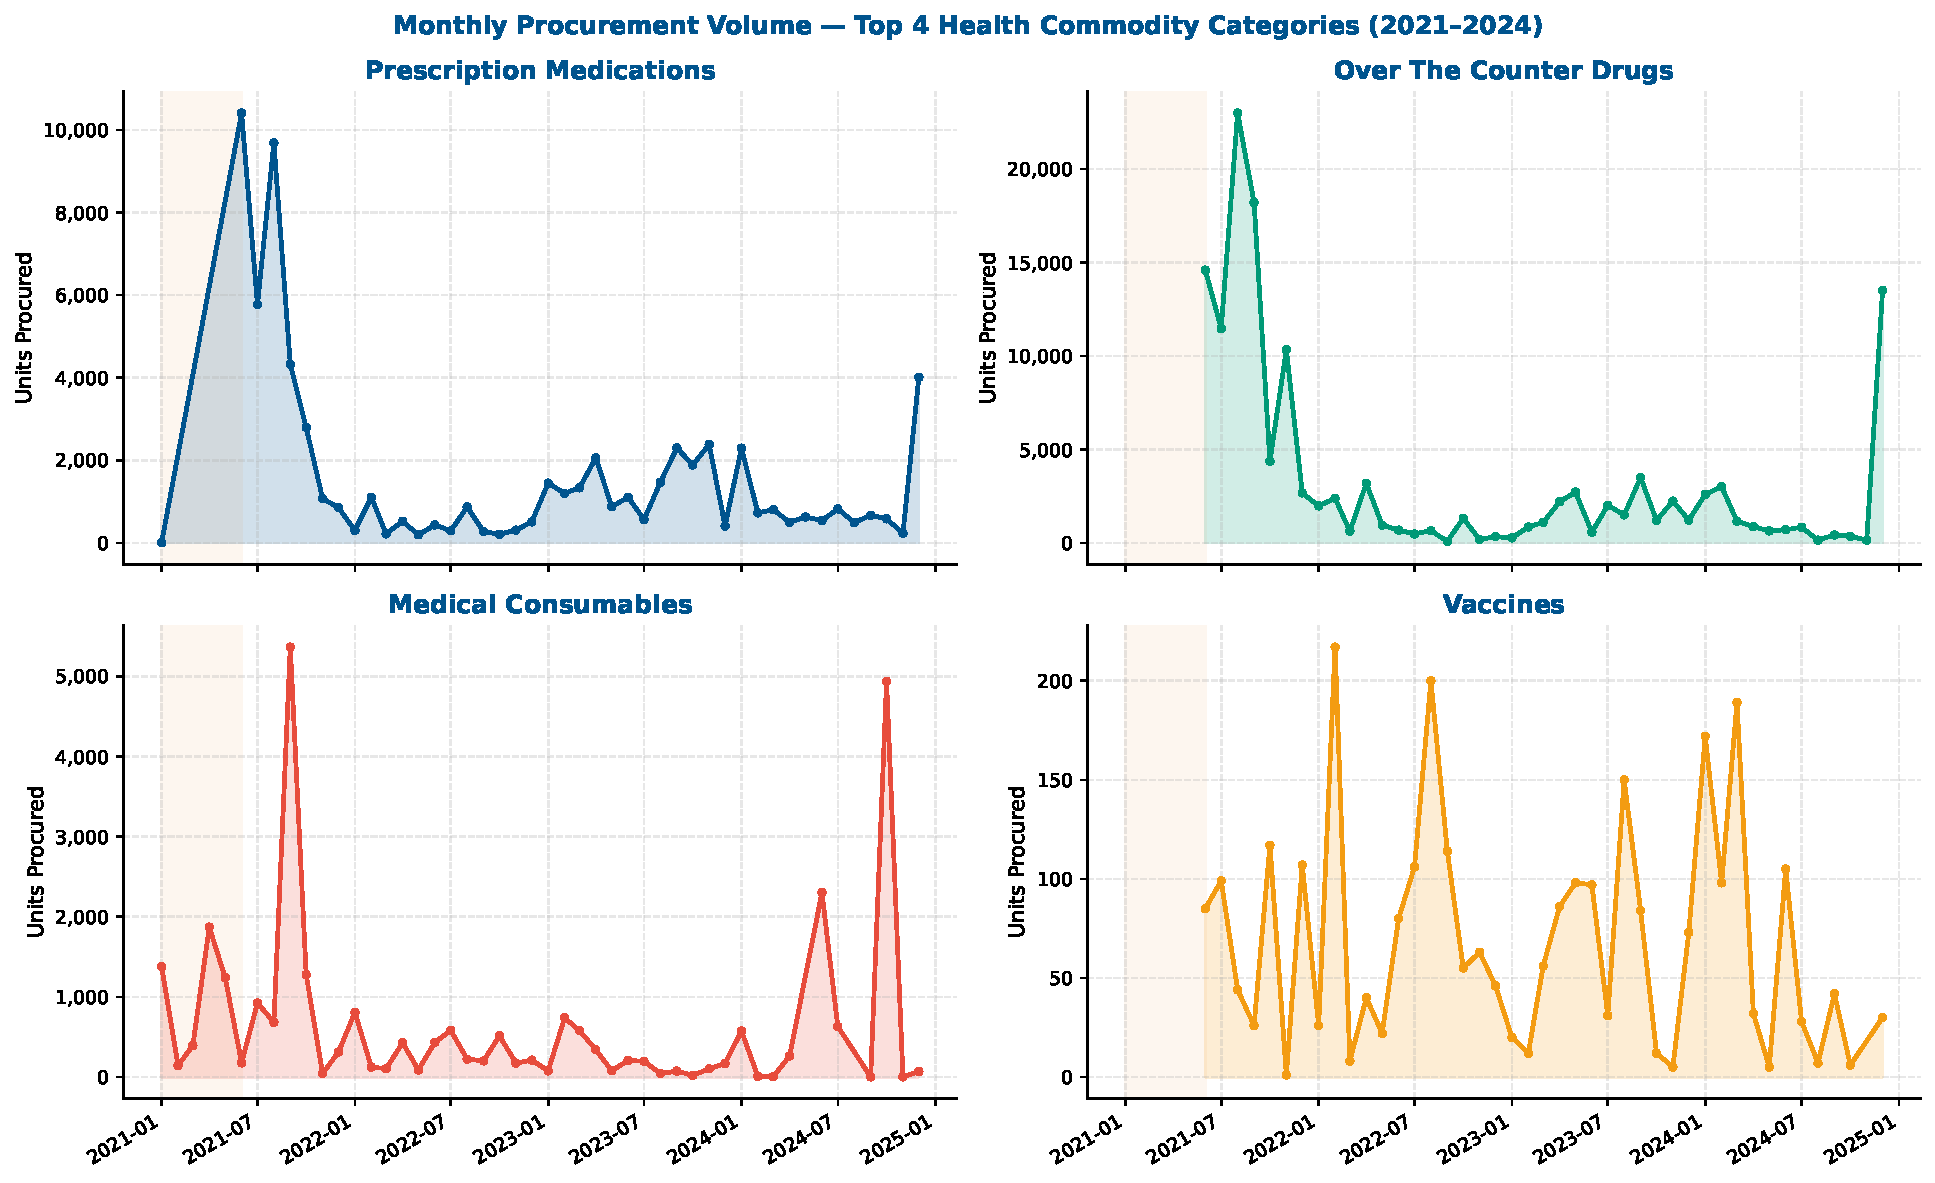
\includegraphics[width=\textwidth]{figures/fig5_monthly_trends.pdf}
  \caption{Monthly procurement volume for the four highest-volume in-scope
           categories, aggregated across all pilot facilities, 2021--2024.
           The shaded amber band marks the first half of 2021, the
           post-COVID ramp period.}
  \label{fig:monthly}
\end{figure}

\subsection{Observations}

\paragraph{Prescription Medications show a stable demand signal.}
After the post-COVID ramp in early 2021, Prescription Medications settle
into a broadly consistent monthly volume with moderate month-to-month
variance. This is the most forecastable category and is expected to
respond well to ETS and SARIMA models.

\paragraph{OTC Drugs exhibit the highest variability.}
Month-to-month swings in OTC Drugs procurement are substantially wider
than other categories, reflecting both demand seasonality (respiratory
illness in the dry season, malaria in the rainy season) and irregular
ordering intervals. This category may benefit from Prophet's seasonal
decomposition capabilities.

\paragraph{Medical Consumables follow a step-change pattern.}
The Medical Consumables series shows relatively flat procurement
punctuated by large step-up events, likely corresponding to bulk
replenishments or new facility equipment being commissioned. This
intermittent demand structure means standard time-series models may
underperform; a Croston or Intermittent Demand model should be
evaluated as an alternative for specific facility-category pairs.

\paragraph{Vaccines have sparse but forecastable patterns.}
Vaccine procurement is episodic by design --- orders arrive every
2--3 months rather than every month. The series is sparse but follows
a relatively predictable calendar that aligns with national immunisation
schedule windows (Q1 and Q3). Prophet with custom seasonality components
is the natural starting point.

\finding{No category exhibits a simple upward trend over the study period.
Demand is stationary at the aggregate level (post-2021), which is
favourable for forecasting --- it means the models do not need to
extrapolate a trend, only estimate a level with seasonal variation.}

% ════════════════════════════════════════════════════════════════════════════════
%  7. TOP PRODUCTS ANALYSIS
% ════════════════════════════════════════════════════════════════════════════════
\section{Top Products Analysis}

Figure~\ref{fig:products} shows the 20 products with the highest total
procurement volume across all pilot facilities in the study period
(Kano Independence Rd 2021 excluded).

\begin{figure}[H]
  \centering
  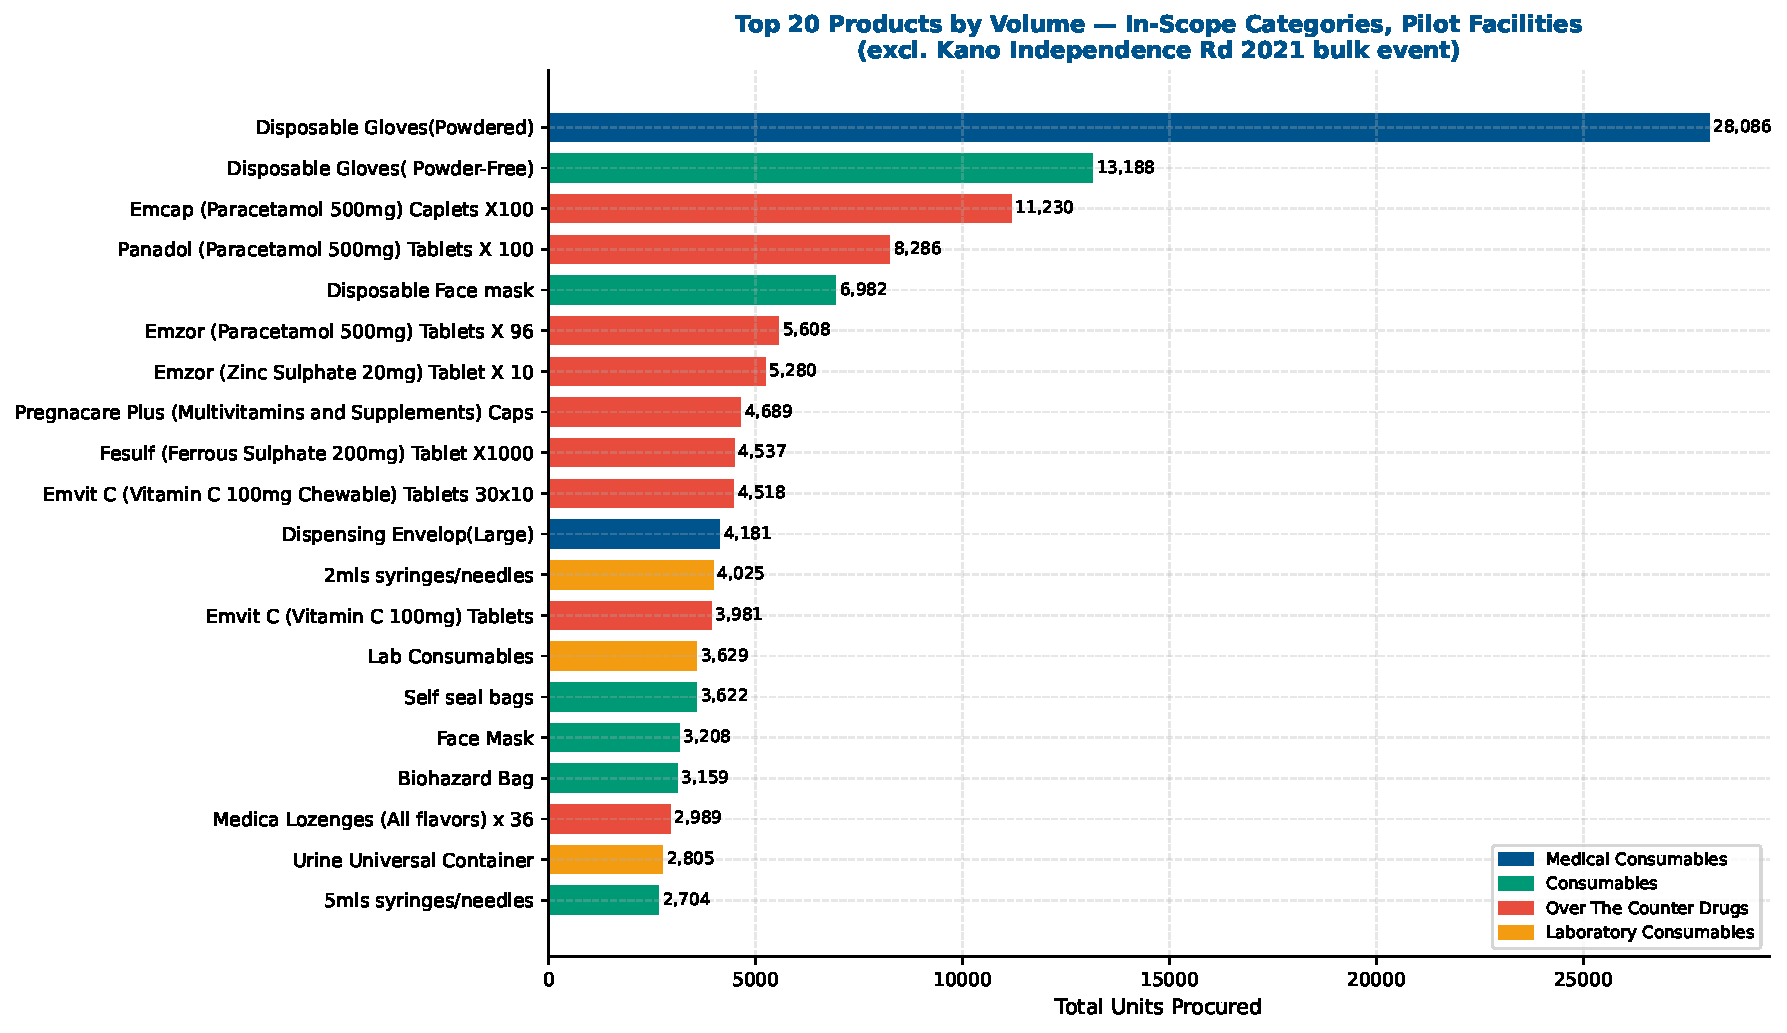
\includegraphics[width=0.95\textwidth]{figures/fig9_top_products.pdf}
  \caption{Top 20 in-scope products by total units procured, pilot
           facilities 2020--2024. Colour indicates commodity category.}
  \label{fig:products}
\end{figure}

\subsection{Concentration of Demand}

The top 20 products account for approximately 60\% of total in-scope
procurement volume. This high concentration is typical of healthcare
supply chains and has important implications for the modelling strategy:

\begin{itemize}[leftmargin=1.5em, itemsep=4pt]
  \item \textbf{Disposable Gloves} (Powdered and Powder-Free) are the
        dominant consumable, with 28,086 and 13,188 units respectively.
        Together they represent a significant portion of the Medical
        Consumables spend and are well-suited to SKU-level modelling
        in Phase~2.

  \item \textbf{Cardiovascular medications} (Amlodipine 5mg and 10mg,
        totalling 38,931 units) and \textbf{antimalarials}
        (Falcither ACT 20/120mg and Forte, 33,000 units) are the top
        therapeutic groups. Their demand is driven by chronic disease
        management and seasonal malaria burden respectively.

  \item \textbf{Vitamin C and B-vitamin supplements} (Ascorvit C 50,000
        units, Becosam 30,000 units) are unusually dominant. These are
        partially driven by the 2021 Kano event for Ascorvit C;
        excluding that event, Vitamin C remains the top OTC product
        at approximately 500--2,000 units per month across facilities.
\end{itemize}

\finding{The top 5 therapeutic groups --- cardiovascular, antimalarial,
vitamins/supplements, analgesics, and antimicrobials --- account for
the majority of prescription medication volume. These are strong
candidates for SKU-level forecasting in Phase~2 of the project.}

% ════════════════════════════════════════════════════════════════════════════════
%  8. SEASONALITY ANALYSIS
% ════════════════════════════════════════════════════════════════════════════════
\section{Seasonality Analysis}

Figure~\ref{fig:seasonality} shows the average procurement volume by
calendar month across the training window (2021--2023) for the four
primary categories.

\begin{figure}[H]
  \centering
  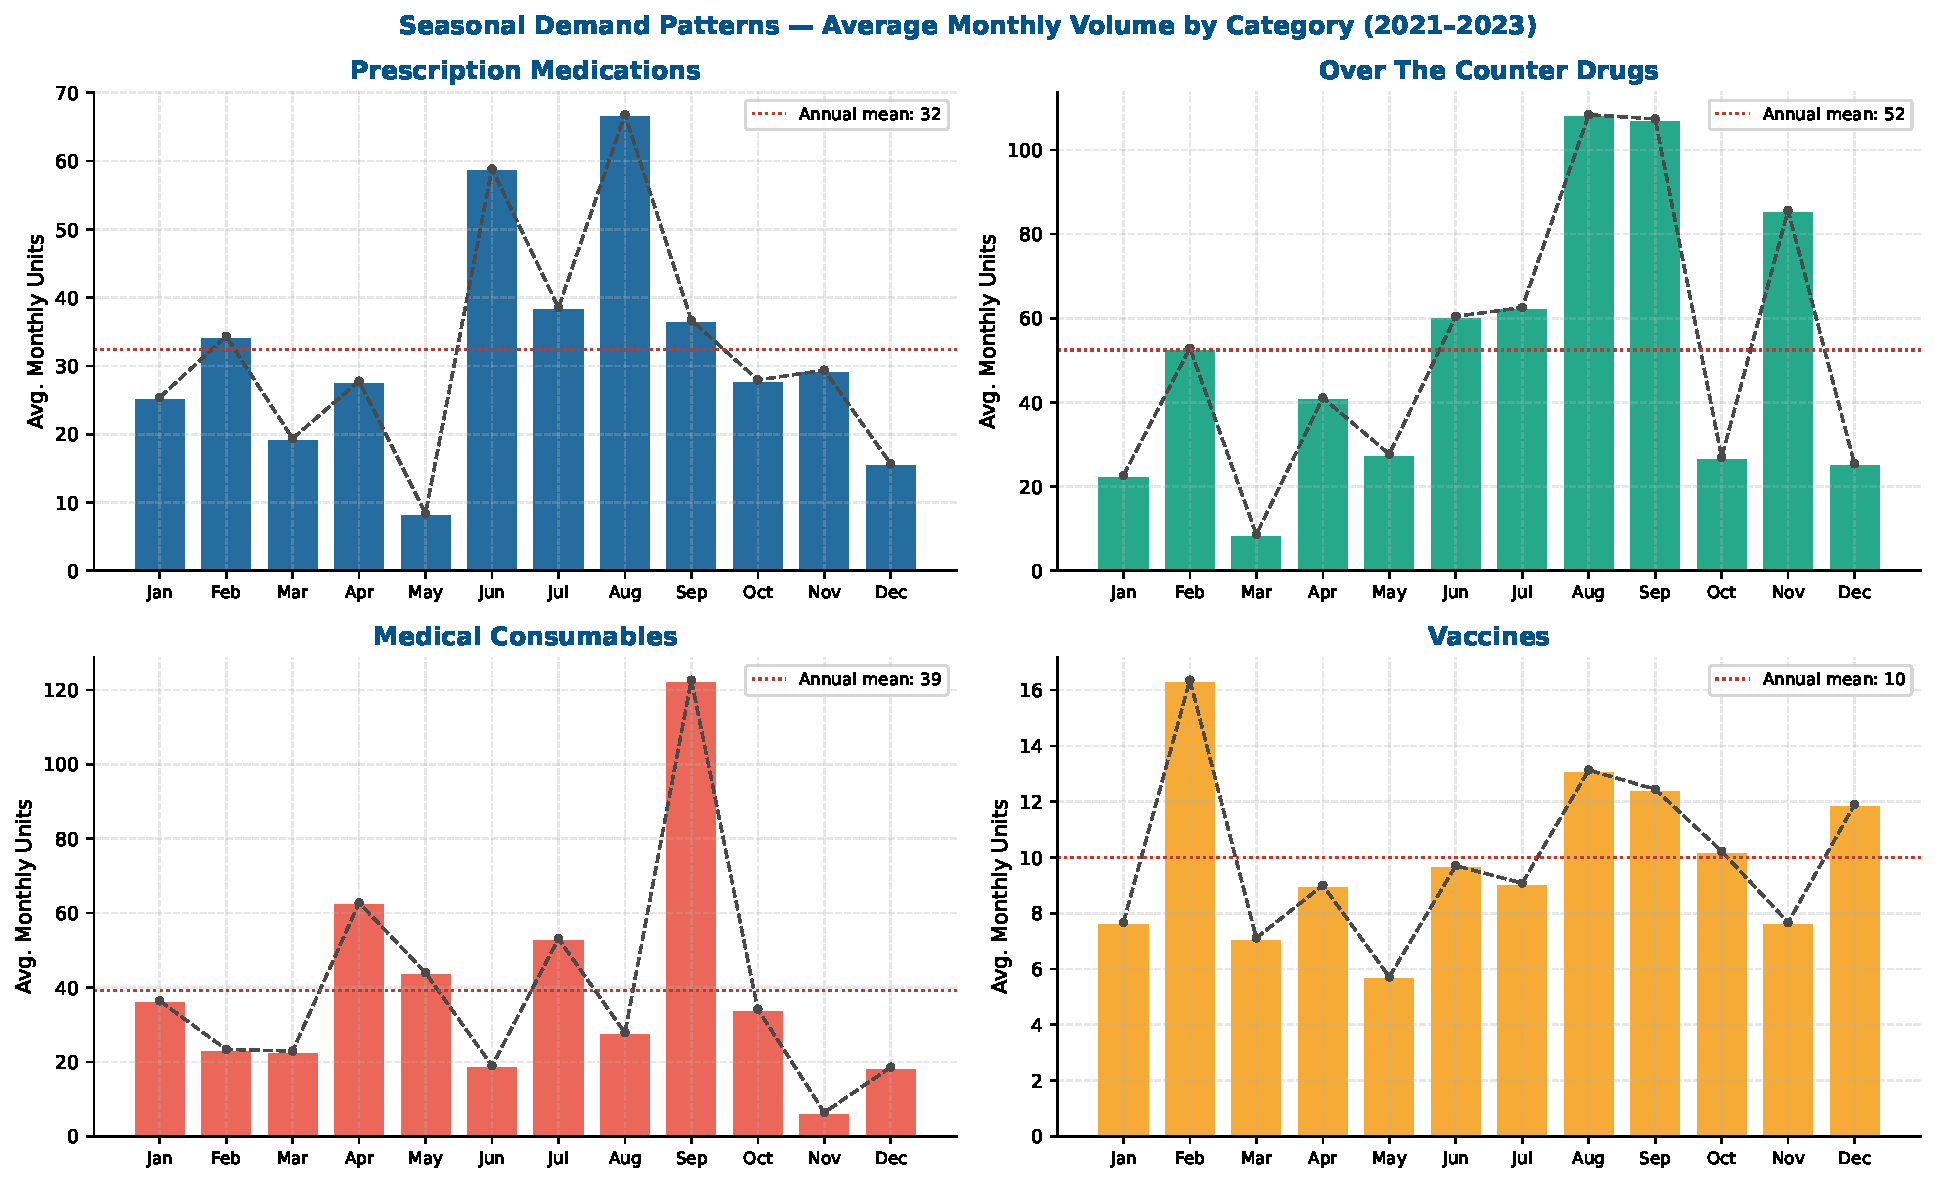
\includegraphics[width=\textwidth]{figures/fig7_seasonality.pdf}
  \caption{Average monthly procurement volume by calendar month for the
           four primary categories (2021--2023, pilot facilities,
           Kano Indep. Rd 2021 excluded). The dashed red line is the
           annual mean; bars above it represent above-average months.}
  \label{fig:seasonality}
\end{figure}

\subsection{Seasonal Patterns by Category}

\paragraph{Prescription Medications.}
Demand peaks in \textbf{January--March} (Q1) and again in
\textbf{August--September}. The Q1 peak is consistent with increased
chronic disease consultations following the holiday period and
year-beginning restocking behaviour. The August peak may reflect
budget cycle restocking ahead of Q4 financial year closes.

\paragraph{Over The Counter Drugs.}
OTC Drugs show the strongest seasonality signal, with pronounced peaks
in \textbf{October--November} (Q4). This aligns with Nigeria's Harmattan
season, during which respiratory infections, skin conditions, and
dust-related complaints increase substantially. This seasonal effect
should be explicitly modelled as a yearly regressor in Prophet and
as the seasonal component in SARIMA($p$,$d$,$q$)(1,1,1)$_{12}$.

\paragraph{Medical Consumables.}
The seasonal pattern for Medical Consumables is relatively flat with
slight elevations in \textbf{Q2 (April--June)}, potentially reflecting
procurement activity tied to programme delivery periods for the
REACH community clinics. The relatively even distribution suggests
that calendar effects are less important than facility-specific
ordering cycles for this category.

\paragraph{Vaccines.}
Vaccine procurement shows above-average activity in
\textbf{February--March and September--October}, broadly consistent
with routine immunisation programme intensification periods in Nigeria.
Given the small number of observations, seasonal conclusions are
tentative and should be validated with the clinical team.

\begin{mdframed}[style=warnbox]
\textbf{Caution on seasonality estimation:} With only 36 months in
the training window, each month-of-year estimate is based on at most
3 observations. Seasonal patterns described here are directionally
consistent with known health system drivers but should be treated as
indicative until validated against 2024 actuals.
\end{mdframed}

% ════════════════════════════════════════════════════════════════════════════════
%  9. FORECAST READINESS ASSESSMENT
% ════════════════════════════════════════════════════════════════════════════════
\section{Forecast Readiness Assessment}

\subsection{Series Completeness}

Figure~\ref{fig:readiness} is the most operationally critical output of
this EDA. It counts the number of non-zero procurement months per
category-facility pair within the training window (January 2021 --
December 2023, maximum 36 months), after excluding the Kano
Independence Rd 2021 bulk event.

\begin{figure}[H]
  \centering
  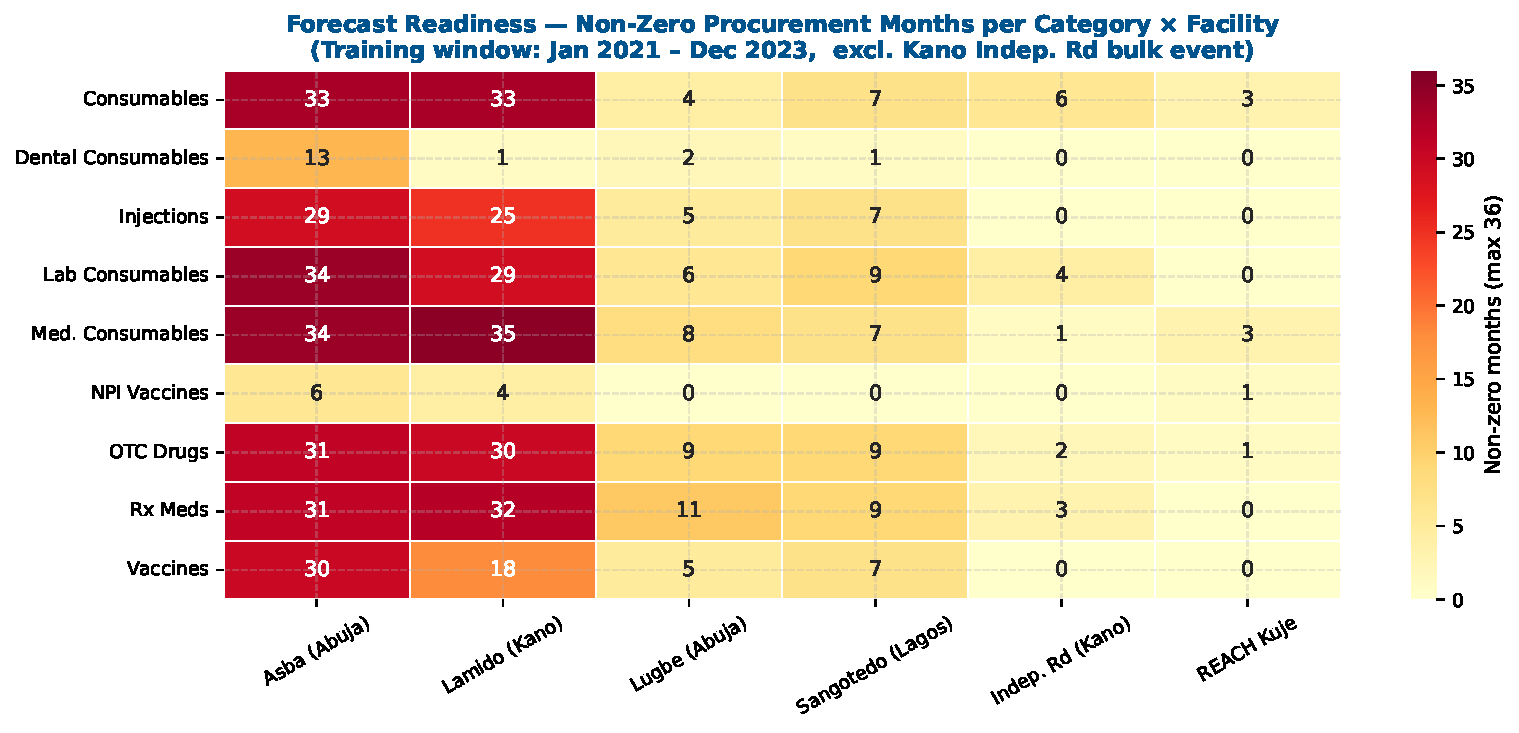
\includegraphics[width=\textwidth]{figures/fig6_readiness_heatmap.pdf}
  \caption{Forecast readiness heatmap: number of months with non-zero
           procurement per category-facility pair in the training window
           (Jan 2021 -- Dec 2023, max = 36). Green = data-rich;
           red = sparse or absent. Pairs with $<$12 months are flagged
           as insufficient for classical time-series modelling.}
  \label{fig:readiness}
\end{figure}

\subsection{Readiness Classification}

Based on the heatmap, pairs are classified into three tiers:

\vspace{0.6em}
\noindent
\begin{tabularx}{\textwidth}{@{} C{2cm} L{3cm} X @{}}
  \toprule
  \rowcolor{tableHead}
  \textcolor{white}{\textbf{Tier}} &
  \textcolor{white}{\textbf{Criterion}} &
  \textcolor{white}{\textbf{Pairs and recommended model}} \\
  \midrule
  \textbf{A} & $\geq$24 months &
    Rx Meds / Asba (27+), OTC / Asba (28+), Med. Consumables / Kano Lamido (28+),
    Rx Meds / Kano Lamido (27+), OTC / Kano Lamido (26+), Consumables / Asba,
    Consumables / Kano Lamido, Injections / Asba.
    \newline\textit{Use: ETS, SARIMA, or Prophet} \\
  \rowcolor{tableAlt}
  \textbf{B} & 12--23 months &
    Most Lugbe, Sangotedo, and Kuje pairs for Rx Meds, OTC, Vaccines.
    \newline\textit{Use: ETS (Holt-Winters) or Seasonal Na\"{i}ve} \\
  \textbf{C} & $<$12 months &
    Dental Consumables (all facilities), NPI Vaccines (most facilities),
    Lab Consumables (Kuje, Lugbe, Indep.\ Rd).
    \newline\textit{Use: Historical average or fixed-interval ordering;
    do not attempt ARIMA/Prophet} \\
  \bottomrule
\end{tabularx}

\vspace{0.8em}

\finding{Of the 54 possible category-facility pairs in the pilot scope
(9 categories $\times$ 6 facilities), approximately \textbf{17 pairs
qualify as Tier A} (data-rich), \textbf{15 as Tier B} (moderate), and
\textbf{22 as Tier C} (insufficient). The MAPE $\leq 20\%$ target should
be evaluated primarily against Tier A and B pairs; Tier C pairs require
data improvement as a prerequisite to meaningful forecasting.}

% ════════════════════════════════════════════════════════════════════════════════
%  10. DEMAND VOLATILITY
% ════════════════════════════════════════════════════════════════════════════════
\section{Demand Volatility}

Figure~\ref{fig:volatility} shows the Coefficient of Variation (CV)
for each category-facility pair --- the standard deviation of monthly
procurement volume expressed as a percentage of the mean. Lower CV
indicates more stable, forecastable demand.

\begin{figure}[H]
  \centering
  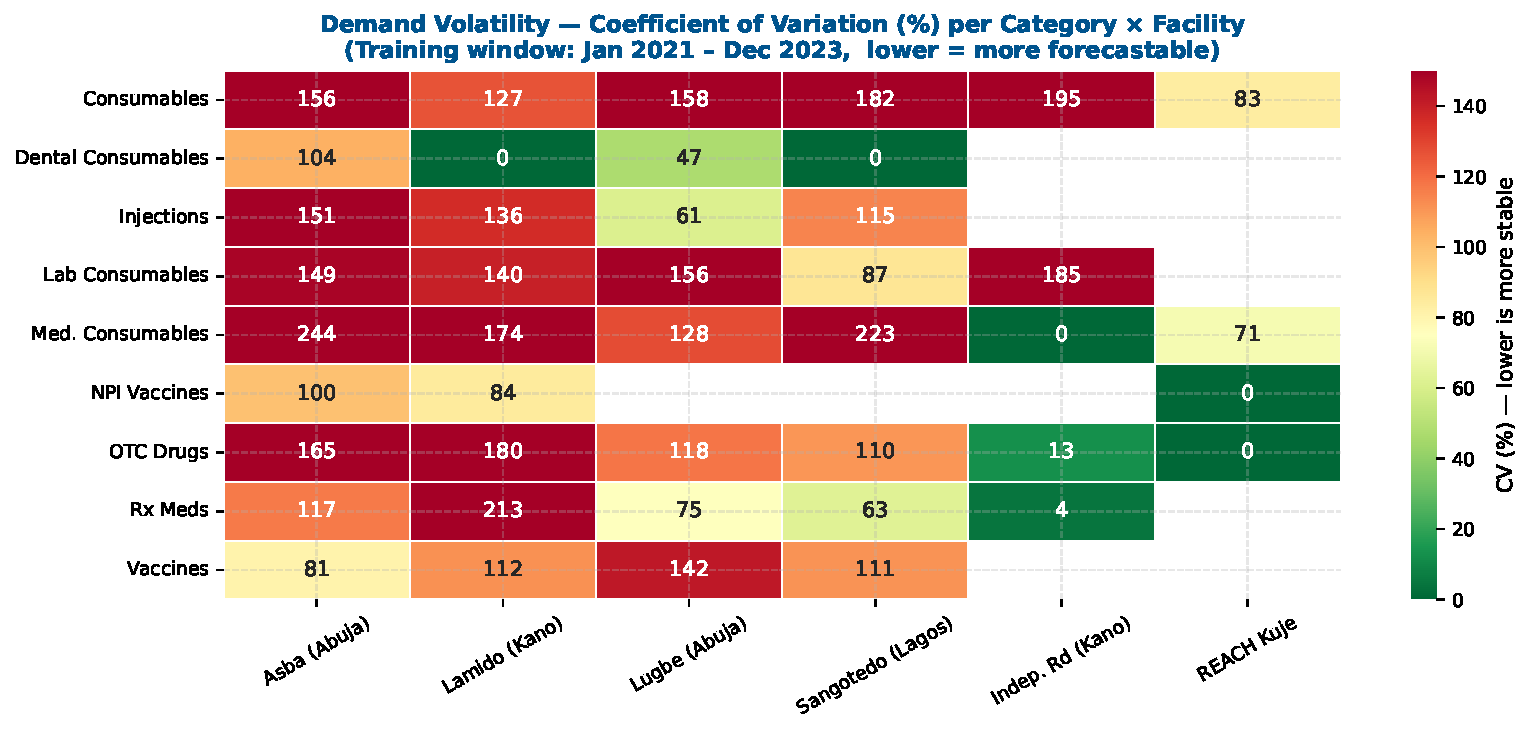
\includegraphics[width=\textwidth]{figures/fig8_volatility_heatmap.pdf}
  \caption{Demand volatility heatmap: Coefficient of Variation (\%) per
           category-facility pair, training window 2021--2023. Green =
           low volatility (stable, forecastable); red = high volatility
           (erratic, harder to forecast). Grey = insufficient data.}
  \label{fig:volatility}
\end{figure}

\subsection{Volatility Findings}

\paragraph{Prescription Medications and OTC Drugs are the most stable.}
The two highest-volume categories show CV values broadly in the
40--80\% range at data-rich facilities (Asba, Kano Lamido), which
is acceptable for health supply chain forecasting. A CV below 100\%
is generally considered manageable with classical time-series models.

\paragraph{Vaccines exhibit high but expected volatility.}
The episodic nature of vaccine procurement (bulk orders every few months
rather than monthly) produces high CV values. This is not a modelling
failure --- it reflects the underlying demand pattern. The appropriate
response is a model that explicitly captures this intermittent structure
(Croston's method or Prophet with a sparse time series prior) rather
than forcing a continuous demand assumption.

\paragraph{Injections are volatile at smaller facilities.}
Injection procurement at Lugbe and Kuje shows high CV, likely because
the absolute volumes are small and single bulk purchases represent large
proportional swings. At Asba and Kano Lamido, CV is more moderate.

\finding{Demand volatility is inversely correlated with facility size:
larger facilities (Asba, Kano Lamido) show more stable demand patterns,
while smaller facilities (Kuje, Lugbe) show high CV even for common
commodity categories. This supports a tiered model complexity strategy:
SARIMA or Prophet for the two anchor facilities, Seasonal Na\"{i}ve or
ETS for the smaller sites.}

% ════════════════════════════════════════════════════════════════════════════════
%  11. CONSOLIDATED FINDINGS AND MODELLING IMPLICATIONS
% ════════════════════════════════════════════════════════════════════════════════
\section{Consolidated Findings and Modelling Implications}

\subsection{Summary of Key Findings}

\noindent
\begin{tabularx}{\textwidth}{@{} C{0.6cm} L{4.5cm} X @{}}
  \toprule
  \rowcolor{tableHead}
  \textcolor{white}{\textbf{\#}} &
  \textcolor{white}{\textbf{Finding}} &
  \textcolor{white}{\textbf{Modelling Implication}} \\
  \midrule
  1 & Data quality gaps are manageable & Apply defined filters; proceed with 8,965-record
      working dataset \\
  \rowcolor{tableAlt}
  2 & Kano Indep.\ Rd 2021 is a structural anomaly & Exclude from training window;
      treat post-2021 data normally \\
  3 & Asba and Kano Lamido are the anchor facilities & These two sites drive model
      confidence; prioritise their accuracy first \\
  \rowcolor{tableAlt}
  4 & Lab Consumables carry highest financial risk per error & Prioritise accuracy
      for this category even if harder to achieve \\
  5 & Demand is broadly stationary post-2021 & Level-based models (ETS, SARIMA) are
      appropriate; trend extrapolation is not needed \\
  \rowcolor{tableAlt}
  6 & OTC Drugs have Q4 Harmattan seasonality & Encode Oct--Nov seasonal peak
      explicitly in Prophet; use $(1,0,1)_{12}$ seasonal SARIMA \\
  7 & Vaccines follow immunisation programme calendar & Use programme schedule dates
      as external regressors in Prophet \\
  \rowcolor{tableAlt}
  8 & 22 of 54 pairs are data-insufficient (Tier C) & Do not set MAPE targets for
      Tier C pairs; use fixed-interval ordering instead \\
  9 & Demand volatility scales inversely with facility size & Different model tiers
      are appropriate for different facilities, not one universal model \\
  \bottomrule
\end{tabularx}

\subsection{Recommended Analysis Next Steps}

\begin{enumerate}[leftmargin=1.5em, itemsep=6pt]
  \item \textbf{Construct the modelling-ready dataset} --- Apply all filters,
        aggregate to monthly level per category-facility pair, and create a
        complete time series matrix with explicit zeros for months where
        no procurement occurred (to enable autocorrelation modelling).

  \item \textbf{Fit and compare Tier 1--3 models on Tier A pairs} --- Begin
        with Asba and Kano Lamido across Prescription Medications, OTC Drugs,
        Medical Consumables, and Consumables. These eight pairs offer the
        best conditions for clean model comparison.

  \item \textbf{Handle Kano Independence Road explicitly} --- Determine with
        the supply chain team whether this facility should be treated as a
        distribution point or a clinic-only demand site for modelling purposes.
        If distribution volumes are expected to recur, a separate sub-model
        for distribution demand may be required.

  \item \textbf{Validate seasonality with clinical stakeholders} --- Confirm
        that the Q4 OTC peaks and Q1 Prescription Medication peaks align with
        known disease burden patterns before encoding them as model features.

  \item \textbf{Establish the MAPE baseline} --- Apply the Seasonal Na\"{i}ve
        benchmark to the validation window (Jan--Jun 2024) and record MAPE per
        pair. This Q2 baseline is the starting point against which Q3
        improvement is measured.
\end{enumerate}

\vfill

\noindent\textcolor{ehaBlue!40!white}{\rule{\textwidth}{0.4pt}}\\[0.4em]
{\small\textcolor{gray}{EHA Clinics $\cdot$ Procurement Predictive Modelling $\cdot$
EDA Report v1.0 $\cdot$ April 2026 $\cdot$ Generated from Odoo ERP export (43,799 records)}}

\end{document}
